\chapter{Modelo matemático}
\cleanchapterquote{En matemáticas no entiendes las cosas, te acostumbras a ellas.}{John von Neumann}{(Físico matemático)}

En el presente capítulo se aborda el modelo matemático que fundamenta el diseño de control en el capítulo 5, pasando por
la definición de los marcos de referencia del sistema, la obtención de sistema dinámico con base en
investigaciones de otros autores.

% ---------------------------------------------------------------------------------------------------------
% *********************************************************************************************************
% *********************************************************************************************************
% ---------------------------------------------------------------------------------------------------------
\section{Marco de referencia}
Hay un concepto clave que ayuda establecer la bases para la comprensión del movimiento de
un cuerpo rígido, que es el de marco de referencia.\\
En la figura 3.1 asociamos con cualquier posición y orientación un marco de referencia
\begin{center}
	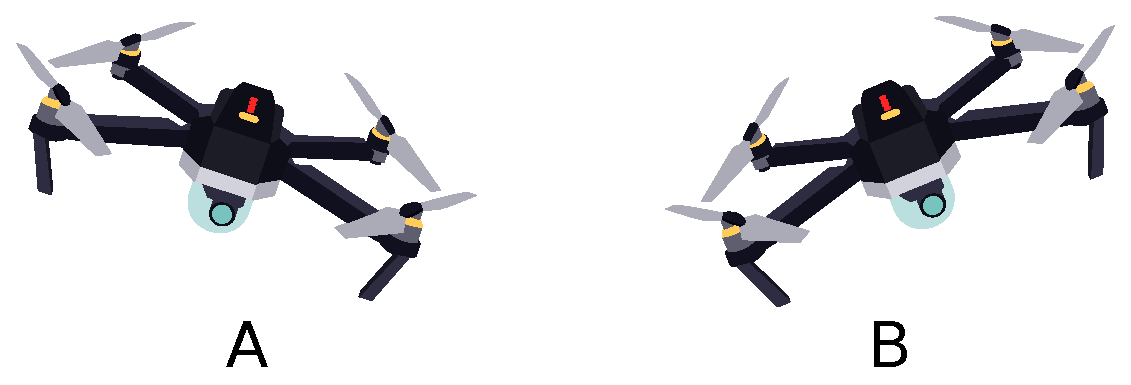
\includegraphics[width=0.55\textwidth]{Contenido/Cuerpo/Capitulo3/Fig10.eps}
	\captionof{figure}{Drone con diferente grado de orientación}
	\label{fig:ModeloMat:Fig1}
\end{center}
En el marco A de la figura 3.2, podemos encontrar 3 vectores linealmente independientes $a_1$, $a_2$ y $a_3$
y de la misma manera en el marco B tenemos tres vectores $b_1$, $b_2$ y $b_3$, podemos
escribir cualquier vector como una combinación lineal del vector base en cualquier marco:
\begin{equation}
	\textbf{v} = v_1 \textbf{a}_1 + v_2 \textbf{a}_2 + v_3 \textbf{a}_3
\end{equation}
Tales vectores pueden ser vistos como ortogonales y si aplicamos una rotación del marco A
la transformación g queda ilustrada en la figura 3.2.
\begin{center}
	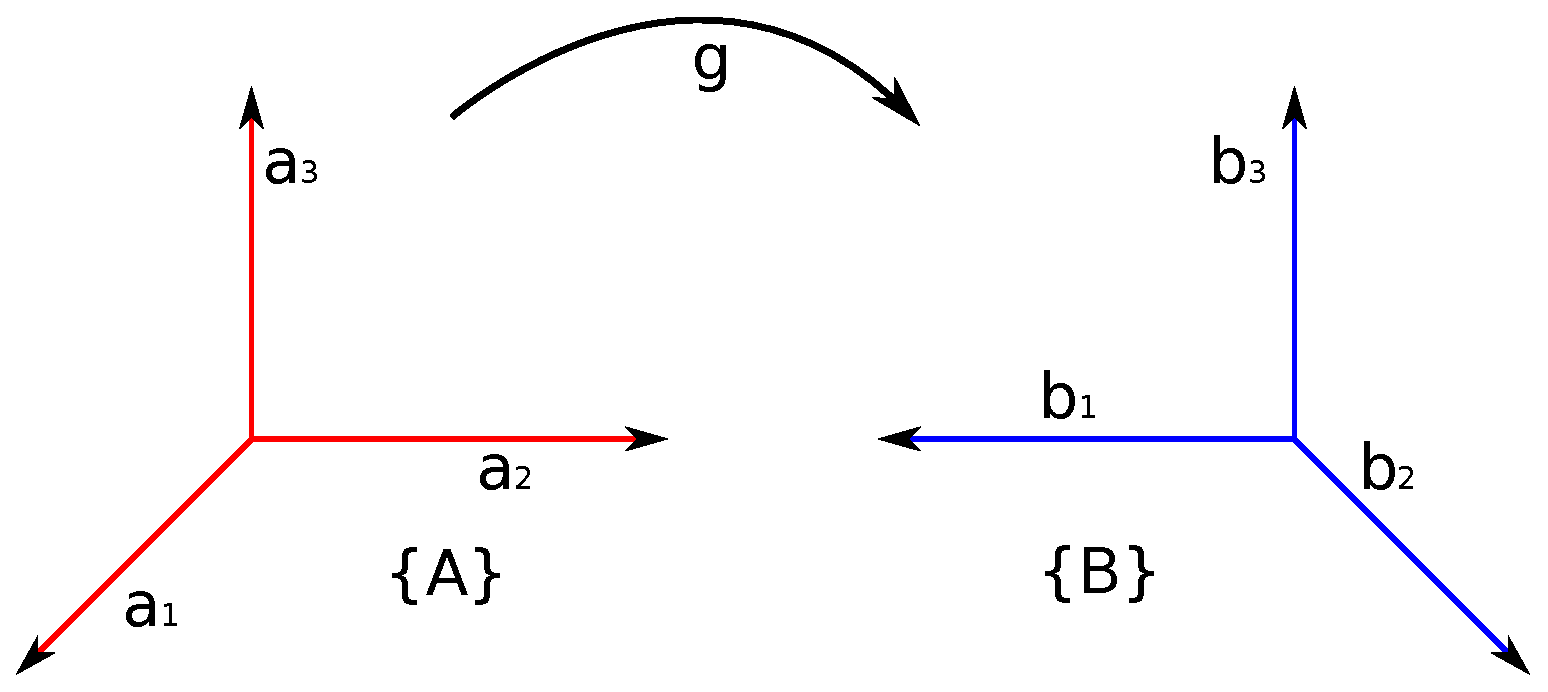
\includegraphics[width=0.55\textwidth]{Contenido/Cuerpo/Capitulo3/Fig11.eps}
	\captionof{figure}{Desplazamiento cuerpo rígido}
	\label{fig:ModeloMat:Fig1}
\end{center}
Podemos escribir ambos vectores ortogonales unitarios en un solo marco de referencia como
una combinación lineal de ambos
\begin{subequations}
	\begin{equation}
		\textbf{b}_1 = R_{11}\textbf{a}_1 + R_{12}\textbf{a}_2 + R_{13}\textbf{a}_3
	\end{equation}
	\begin{equation}
		\textbf{b}_2 = R_{21}\textbf{a}_1 + R_{22}\textbf{a}_2 + R_{23}\textbf{a}_3
	\end{equation}
	\begin{equation}
		\textbf{b}_3 = R_{31}\textbf{a}_1 + R_{32}\textbf{a}_2 + R_{33}\textbf{a}_3
	\end{equation}
\end{subequations}
Para este caso se escoge \textbf{b}$_1$, \textbf{b}$_2$ y \textbf{b}$_3$ como la combinación
lineal para \textbf{a}$_1$, \textbf{a}$_2$ y \textbf{a}$_3$ y los coeficientes de R se
pueden acomodar en un arreglo de 3x3 llamada matriz de rotación.
\begin{equation}
	R=
	\begin{bmatrix}
		R_{11} & R_{12} & R_{13} \\
		R_{21} & R_{22} & R_{23} \\
		R_{31} & R_{32} & R_{33}
	\end{bmatrix}
\end{equation}
Y las propiedades de esta matriz son las siguientes
\begin{itemize}
	\item Ortogonal
	\item Su determinante es +1
	\item El producto de dos matrices de rotación da como resultado otra matriz de rotación
	\item La inversa de una matriz de rotación es también una matriz de rotación
\end{itemize}
La importancia de las matrices de rotación radican en que con ayuda de software y hardware
podemos aplicar técnicas de mapeo y simulación, además de que para el sistema de la gimbal
entra en juego múltiples marcos de referencia que constantemente cambian su orientación y
desplazamiento.\\
Ahora bien si trazamos un vector Q en cada marco de referencia como en la figura 3.3
\begin{center}
	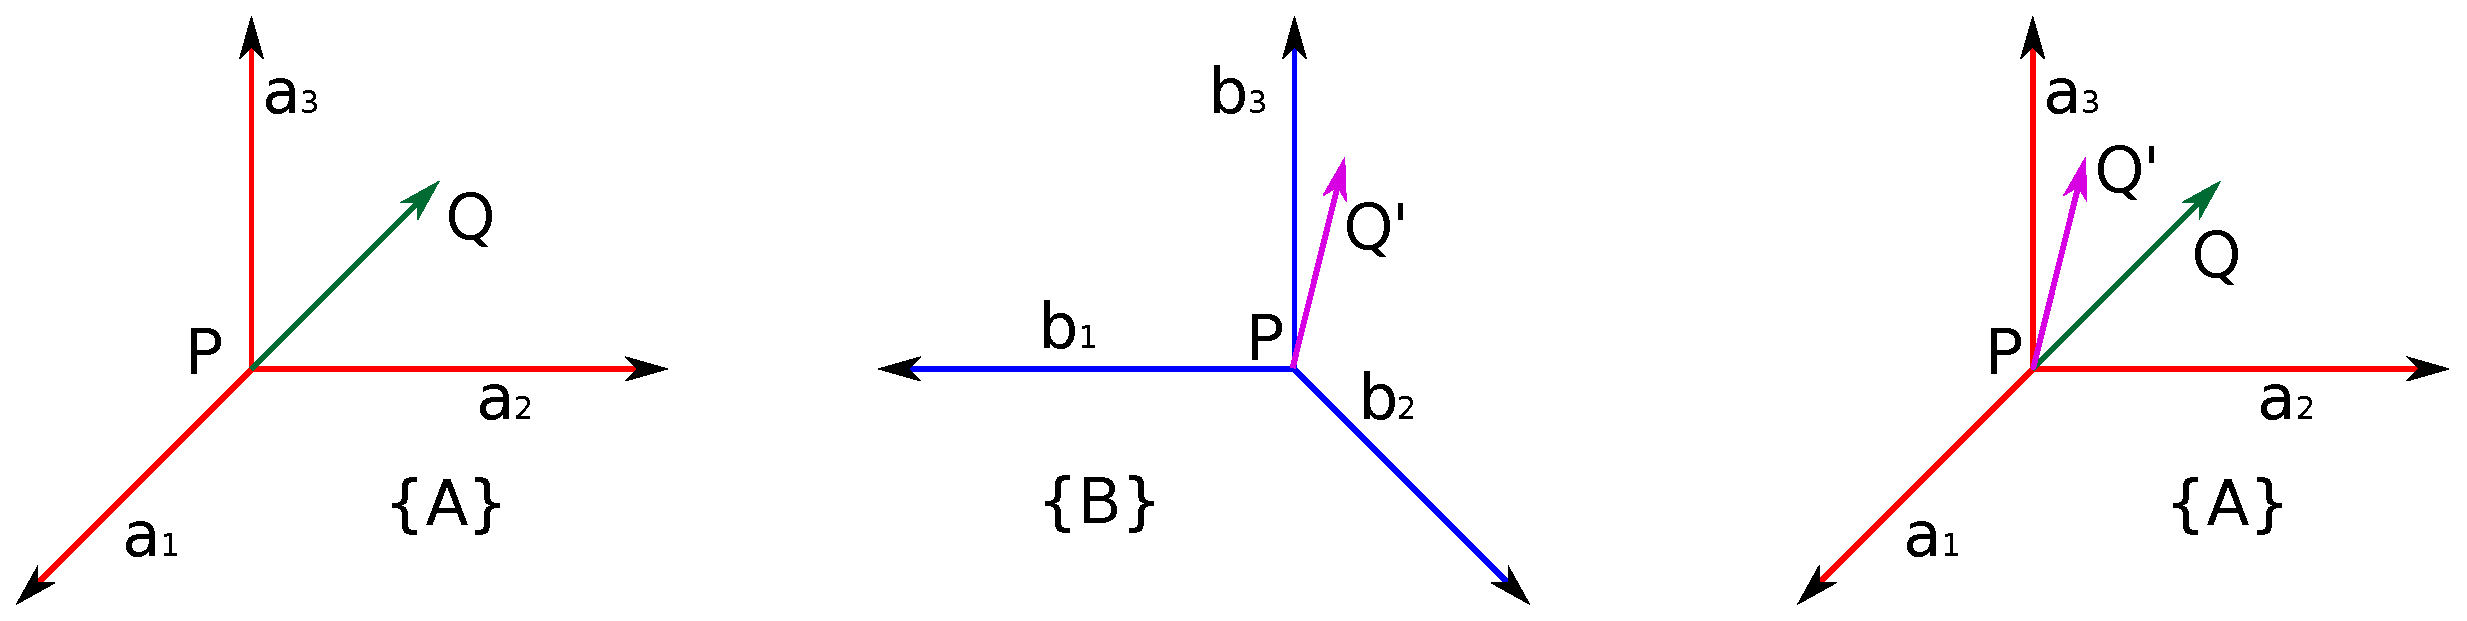
\includegraphics[width=0.85\textwidth]{Contenido/Cuerpo/Capitulo3/Fig12.eps}
	\captionof{figure}{Vectores de rotación}
	\label{fig:ModeloMat:Fig1}
\end{center}
Si trasladamos el marco B en A podremos obtener de nuevo una combinación lineal pero con
diferentes conjuntos de coeficientes
\begin{equation}
	\overrightarrow{PQ} = q_1\textbf{a}_1 + q_2\textbf{a}_2 + q_3\textbf{a}_3
\end{equation}
\begin{equation}
	\overrightarrow{PQ'} = q'_1\textbf{a}_1 + q'_2\textbf{a}_2 + q'_3\textbf{a}_3
\end{equation}
La matriz que conecta $q_1$, $q_2$ y $q_3$ con $q'_1$ , $q'_2$ y $q'_3$ es la matriz de
rotación vista en la ecuación 3.3
\begin{equation}
	\begin{bmatrix}
		q_1 \\
		q_2 \\
		q_3
	\end{bmatrix}
	=
	\begin{bmatrix}
		R_{11} & R_{12} & R_{13} \\
		R_{21} & R_{22} & R_{23} \\
		R_{31} & R_{32} & R_{33}
	\end{bmatrix}
	\begin{bmatrix}
		q'_1 \\
		q'_2 \\
		q'_3
	\end{bmatrix}
\end{equation}
Dicha matriz nos dice como se transforman los vectores de un marco de referencia a otro. La matrices
de rotación nos van a servir, como se mencionó anteriormente, para poder hacer mapeos del entorno, por
lo que necesitamos primero definir los marcos de referencia inercial y del cuerpo para posteriormente
hacer sus matrices de transformación.

\subsection{Marco de referencia Inercial [I]}
Antes de abordar el control de la gimbal, es necesario y obvio conocer el comportamiento
de dicho sistema, empezaremos por definir el marco de referencia inercial, es decir
el de la tierra. La Figura 3.4 ilustra los ejes de este marco.
\begin{center}
	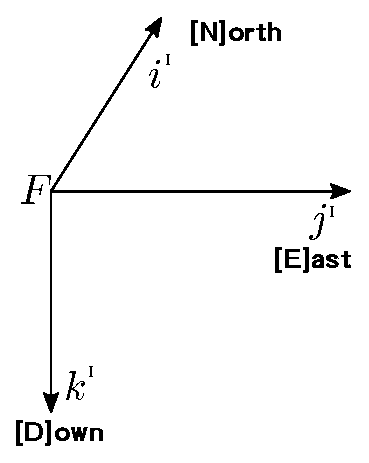
\includegraphics[width=0.25\textwidth]{Contenido/Cuerpo/Capitulo3/Fig4.eps}
	\captionof{figure}{Marco de referencia inercial}
	\label{fig:ModeloMat:Fig1}
\end{center}
Donde definimos a k apuntando hacia el centro de la tierra, este sistema de coordenadas
refieren a (Norte, Este y Abajo) de ahí su nombre NED(siglas en inglés).

\subsection{Marco de referencia del cuerpo [B]}
Una aeronave tiene la libertad de rotar en 3 ejes, en la aeronáutica son conocidos como
Yaw, Pitch y Roll. Dichas rotaciones son importantes en el control de aeronaves ya
que sirven para conocer la dinámica del sistema, dichas rotaciones pueden ser mejor
detalladas en una imagen, por lo que en la ilustración 3.5 se grafica un plano 2D
y se asigna nombre a cada rotación de los ejes.
\begin{center}
	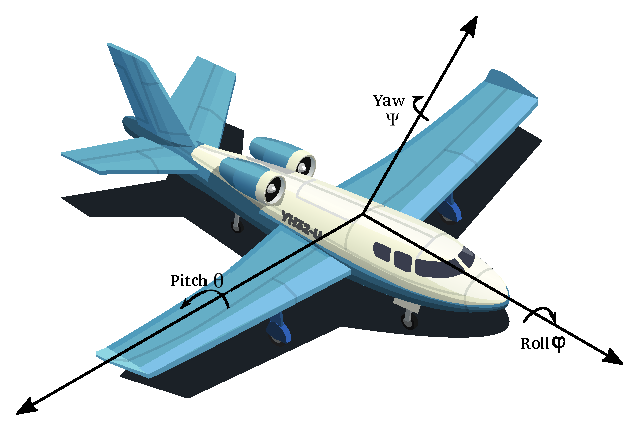
\includegraphics[width=0.65\textwidth]{Contenido/Cuerpo/Capitulo3/Fig6.eps}
	\captionof{figure}{Rotación en 3 ejes.Tomada de freepik}
	\label{fig:ModeloMat:Fig1}
\end{center}
Vamos a llamar marco de referencia del cuerpo a las coordenadas del UAV, es necesario establecer el centro del plano en el
centro de masas de la aeronave, como se ilustra en la figura 3.6.
\begin{center}
	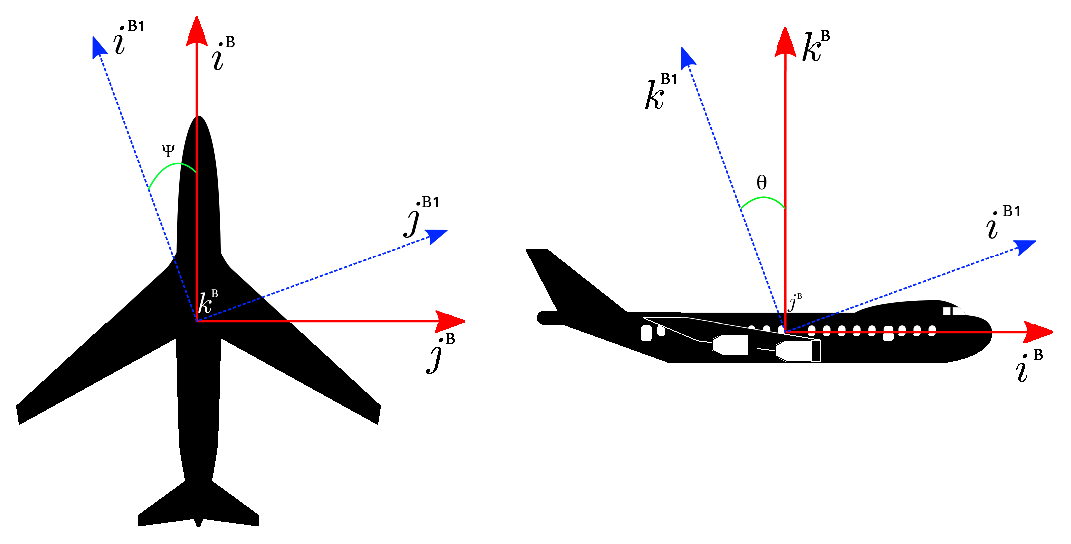
\includegraphics[width=0.9 \textwidth]{Contenido/Cuerpo/Capitulo3/Fig5.eps}
	\captionof{figure}{Marco de referencia del cuerpo.}
	\label{fig:ModeloMat:Fig1}
\end{center}
De donde definimos las dos rotaciones que serán controladas en este trabajo pitch y yaw($\theta$, $\psi$). El subíndice B hace referencia
a Body y nos indica que estamos hablando de las coordenadas del UAV.

\subsection{Marco de referencia de la gimbal [G]}
Un último paso es definir un marco de referencia para la cámara, considerando que la cámara se encuentra en la parte delantera de
la aeronave y que el centro de la gimbal es el origen.
\begin{center}
	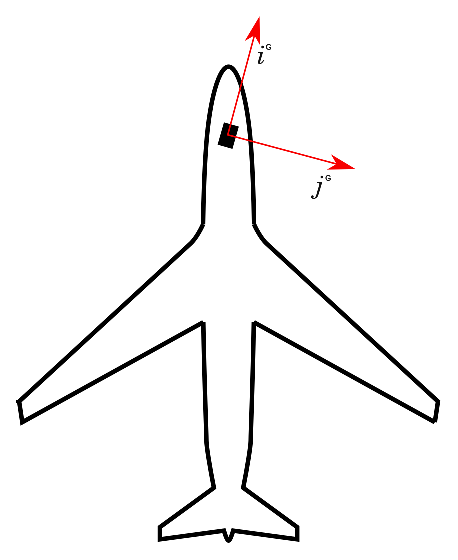
\includegraphics[width=0.5\textwidth]{Contenido/Cuerpo/Capitulo3/Fig7.eps}
	\captionof{figure}{Marco de referencia del la cámara.}
	\label{fig:ModeloMat:Fig1}
\end{center}
De donde el subíndice G hace referencia a que estamos en el plano de la gimbal. El vector unitario K apunta hacia afuera,
es decir hacia nosotros.

% ---------------------------------------------------------------------------------------------------------
% *********************************************************************************************************
% *********************************************************************************************************
% ---------------------------------------------------------------------------------------------------------

\section{Matrices de rotación}
Considerando el marco de referencia del cuerpo(B) y el de la Gimbal(G) tenemos los puntos Q y Q'
Como se ilustra en la figura 3.8.
\begin{center}
	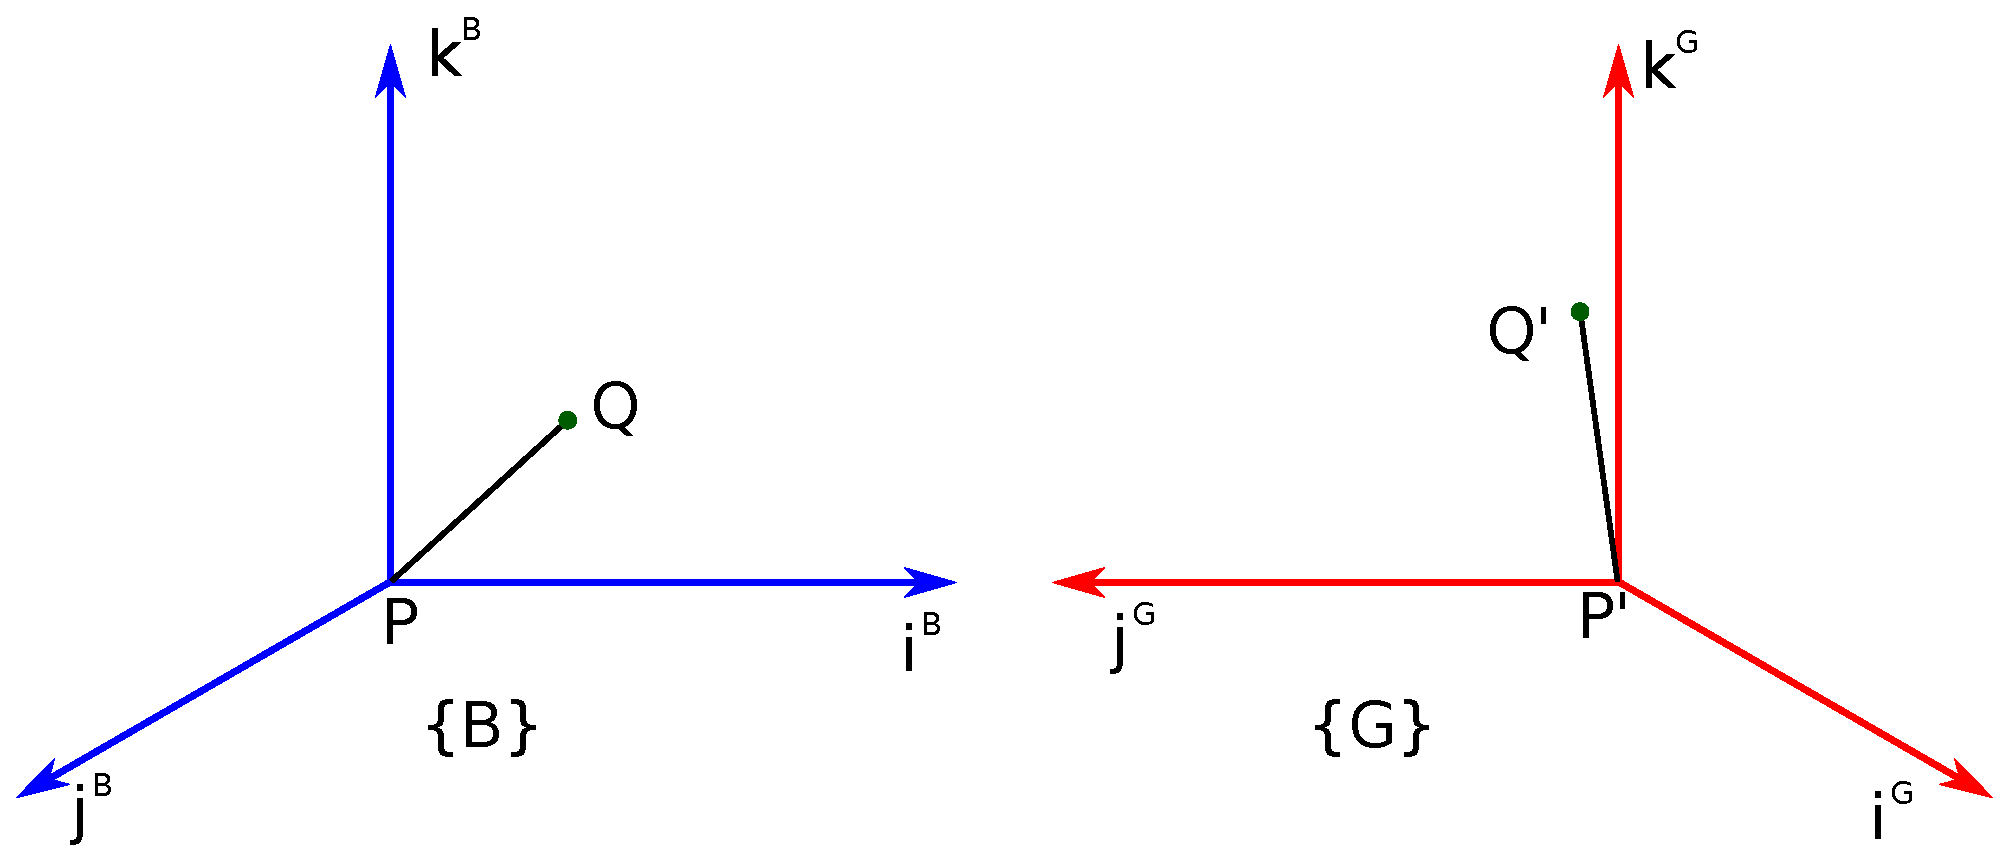
\includegraphics[width=0.75\textwidth]{Contenido/Cuerpo/Capitulo3/Fig13.eps}
	\captionof{figure}{Marco de referencia Body y gimbal}
	\label{fig:ModeloMat:Fig1}
\end{center}
Que podemos expresarlo en una combinación lineal para $\overrightarrow{PQ}$ y para $\overrightarrow{P'Q'}$
\begin{subequations}
	\begin{equation}
		PQ = q_1i^B + q_2j^B + q_3k^B
	\end{equation}
	\begin{equation}
		P'Q' = q_1i^G + q_2j^G + q_3k^G
	\end{equation}
\end{subequations}
Trasladamos el marco de referencia del gimbal en el del cuerpo
\begin{center}
	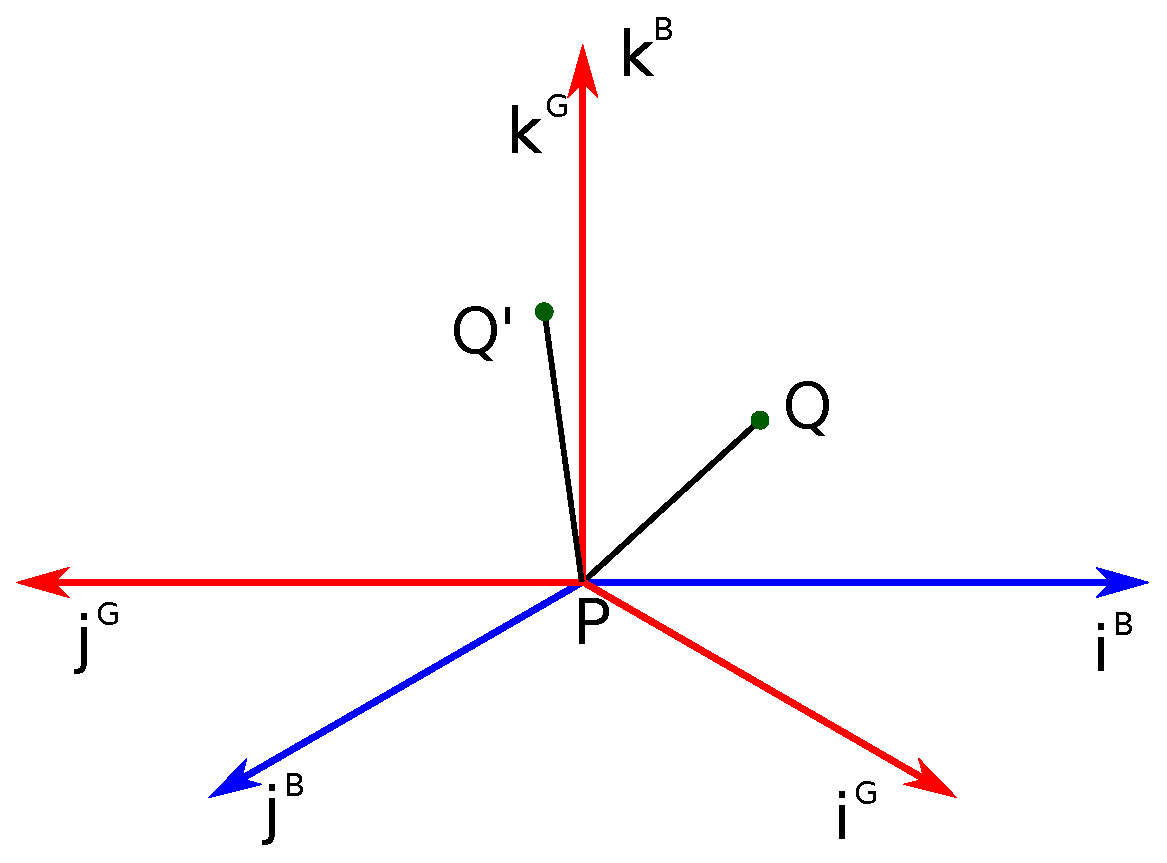
\includegraphics[width=0.45\textwidth]{Contenido/Cuerpo/Capitulo3/Fig14.eps}
	\captionof{figure}{Marco de referencia del gimbal trasladado en el del cuerpo}
	\label{fig:ModeloMat:Fig1}
\end{center}
Ahora tenemos un punto Q'' que es el punto Q' trasladado en el marco de referencia del cuerpo
\begin{equation}
	PQ'' = q_1i^B + q_2j^B + q_3k^B = q_1''i^G + q_2''j^G + q_3''k^G
\end{equation}
\begin{equation}
	\begin{bmatrix}
		q_1'' \\
		q_2'' \\
		q_3''
	\end{bmatrix}
	=
	\begin{bmatrix}
		R_{11} & R_{12} & R_{13} \\
		R_{21} & R_{22} & R_{23} \\
		R_{31} & R_{32} & R_{33}
	\end{bmatrix}
	\begin{bmatrix}
		q_1 \\
		q_2 \\
		q_3
	\end{bmatrix}
\end{equation}
La rotación sobre el eje k se ilustra en la figura 3.10.
\begin{center}
	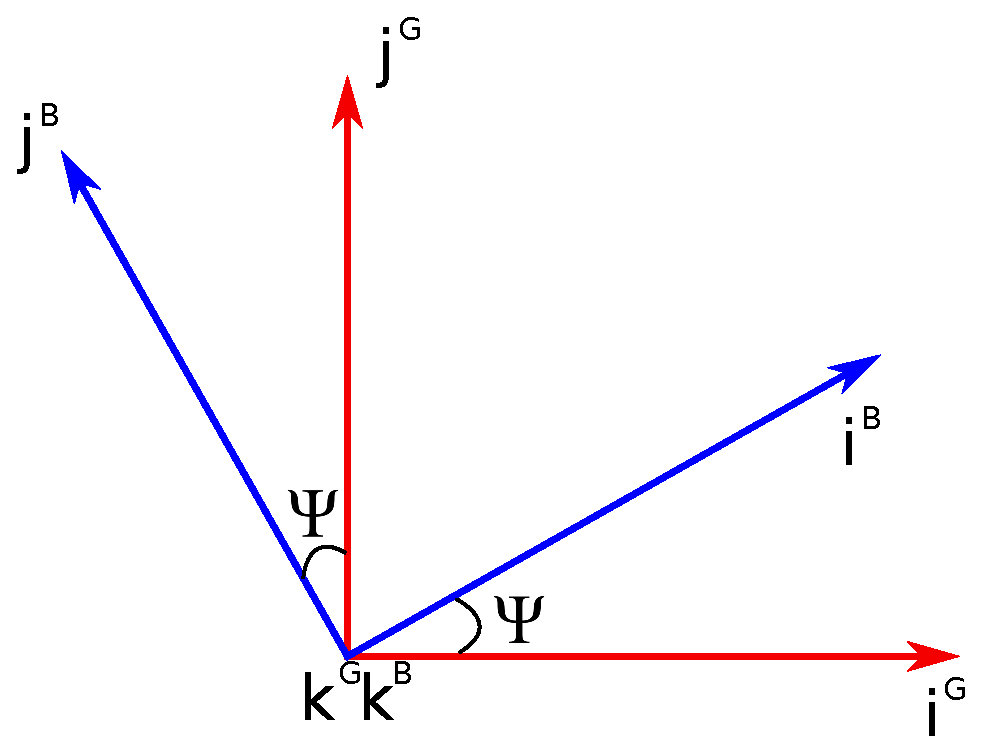
\includegraphics[width=0.45\textwidth]{Contenido/Cuerpo/Capitulo3/Fig15.eps}
	\captionof{figure}{Rotación en el eje k}
	\label{fig:ModeloMat:Fig1}
\end{center}
Se obtiene el cambio para $j^B$ y $i^B$
\begin{equation}
	i^B = |i^B|cos(\psi)i^G + |i^B|sin(\psi)j^G = cos(\psi)i^G + sin(\psi)j^G
\end{equation}
\begin{equation}
	j^B = -|j^B|sin(\psi)i^G + |j^B|cos\psi)j^G = -sin(\psi)i^G + cos(\psi)j^G
\end{equation}
Y de la ecuación 3.8 sustituimos $j^B$ y $i^B$
\begin{equation}
	PQ'' = q_1(cos(\psi)i^G + sin(\psi)j^G) + q_2(-sin(\psi)i^G + cos(\psi)j^G) + q_3(k^G)
\end{equation}
Simplificando la ecuación 3.12 tenemos
\begin{equation}
	PQ''= (q_1cos(\psi) - q_2sin(\psi))i^G + (q_1sin(\psi) + q_2cos(\psi))j^G + q_3(k^G)
\end{equation}
Y acomodando la ecuación 3.13 en matrices tenemos
\begin{equation}
	\begin{bmatrix}
		q_1'' \\
		q_2'' \\
		q_3''
	\end{bmatrix}
	=
	\begin{bmatrix}
		cos(\psi) & -sin(\psi) & 0 \\
		sin(\psi) & cos(\psi)  & 0 \\
		0         & 0          & 1
	\end{bmatrix}
	\begin{bmatrix}
		q_1 \\
		q_2 \\
		q_3
	\end{bmatrix}
\end{equation}
Ahora si rotamos sobre el eje x como se muestra en la figura 3.11
\begin{center}
	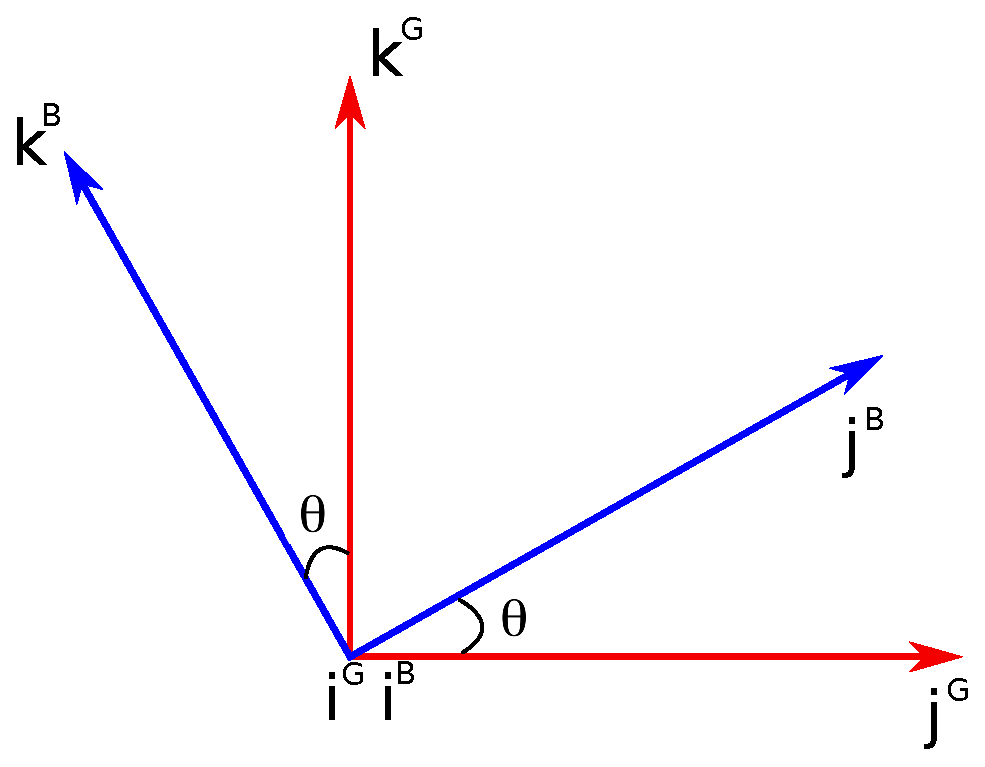
\includegraphics[width=0.45\textwidth]{Contenido/Cuerpo/Capitulo3/Fig17.eps}
	\captionof{figure}{Rotación en el eje x}
	\label{fig:ModeloMat:Fig1}
\end{center}
Se obtiene el cambio para $j^B$ y $k^B$
\begin{equation}
	j^B = |j^B|cos(\theta)j^G + |j^B|sin(\theta)k^G = cos(\theta)j^G + sin(\theta)k^G
\end{equation}
\begin{equation}
	k^B = -|k^B|sin(\theta)j^G + |k^B|cos\theta)k^G = -sin(\theta)j^G + cos(\theta)k^G
\end{equation}
Y de la ecuación 3.8 sustituimos $j^B$ y $k^B$
\begin{equation}
	PQ'' = q_1(i^G) + q_2(cos(\theta)j^G + sin(\theta)k^G) + q_3(-sin(\theta)j^G + cos(\theta)k^G)
\end{equation}
Simplificando la ecuación 3.18 tenemos
\begin{equation}
	PQ''= q_1(i^G) + (q_2cos(\theta) - q_3sin(\theta))j^G + (q_2sin(\theta) + q_3cos(\theta))k^G
\end{equation}
Y acomodando la ecuación 3.18 en matrices tenemos
\begin{equation}
	\begin{bmatrix}
		q_1'' \\
		q_2'' \\
		q_3''
	\end{bmatrix}
	=
	\begin{bmatrix}
		1 & 0           & 0            \\
		0 & cos(\theta) & -sin(\theta) \\
		0 & sin(\theta) & cos(\theta)
	\end{bmatrix}
	\begin{bmatrix}
		q_1 \\
		q_2 \\
		q_3
	\end{bmatrix}
\end{equation}

% ---------------------------------------------------------------------------------------------------------
% *********************************************************************************************************
% *********************************************************************************************************
% ---------------------------------------------------------------------------------------------------------

\section{Ecuaciones de movimiento de una gimbal}
Tres marcos de referencia han sido introducidos en este capítulo; el del cuerpo[B], el de la gimbal[G] y el inercial[I]. Podemos
dividir el marco de referencia de la gimbal en dos: Yaw[K] y Pitch[P], tal y como se ilustra en la figura 3.12.
\begin{center}
	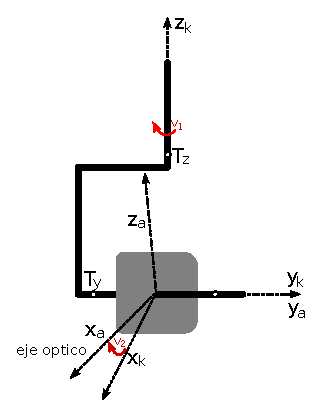
\includegraphics[width=0.4\textwidth]{Contenido/Cuerpo/Capitulo3/Fig20.eps}
	\captionof{figure}{Sistema gimbal de dos grados de libertad}
	\label{fig:ModeloMat:Fig1}
\end{center}
El eje $x_a$ coincide con el eje óptico de la cámara, el centro de rotación está en el origen del marco de referencia, que asumimos es el mismo para los tres marcos.\\
Podemos expresar las velocidades angulares de los marcos de referencia B,K y A en matrices de 3x1.
\begin{equation}
	\begin{bmatrix}
		p \\
		q \\
		r
	\end{bmatrix};
	\begin{bmatrix}
		p_k \\
		q_k \\
		r_k
	\end{bmatrix};
	\begin{bmatrix}
		p_a \\
		q_a \\
		r_a
	\end{bmatrix}
\end{equation}
Y el tensor de inercia para Pitch lo definimos como:
\begin{equation}
	J_A =
	\begin{bmatrix}
		J_{ax} & D_{xy} & D_{xz} \\
		D_{xy} & J_{ay} & D_{yz} \\
		D_{xz} & D_{yz} & J_{az}
	\end{bmatrix}
\end{equation}
Mientras que para Yaw tenemos
\begin{equation}
	J_K =
	\begin{bmatrix}
		J_{kx} & d_{xy} & d_{xz} \\
		d_{xy} & J_{ky} & d_{yz} \\
		d_{xz} & d_{yz} & J_{kz}
	\end{bmatrix}
\end{equation}
Para el signo de los productos de inercia, seguimos la definición de \cite{Book:Goldstein1980}; en consecuencia, no se utilizan explícitamente signos negativos en las matrices.
Se supone que el centro de masa de la gimbal está en el centro de rotación común, es decir, asumimos que la gimbal no tienen desequilibrio de masa.\\
En la figura 3.12 se ilustra los dos torques de entrada del sistema\\
\begin{center}
	$T_y$ = El torque alrededor del eje $Y_a$\\
	$T_y$ = El torque alrededor del eje $Z_k$
\end{center}

\subsection{Rotación sobre Pitch}
La ecuación básica del movimiento en Pitch de la gimbal se obtiene directamente si pensamos en la gimbal como un cuerpo rígido por sí mismo y consideramos el hecho de que no
hay desequilibrio, y recordando que el momento de Inercia es la resistencia que presenta un cuerpo a ser acelerado en rotación podemos hacer una analogía de la segunda
ley de Newton equivalente para la rotación.
\begin{equation}
	\tau = I\alpha
\end{equation}
Donde
\begin{itemize}
	\item $\tau$ es el torque Aplicando.
	\item $I$ es el momento de inercia.
	\item $\alpha$ es la aceleración angular
\end{itemize}
Recordando que el momento angular puede ser calculado mediante la ecuación
\begin{equation}
	H=J\omega
\end{equation}
Por lo que para Pitch tenemos
\begin{equation}
	H_A=
	\begin{bmatrix}
		J_{ax}p_a + D_{xy}q_a + D_{yz}r_a \\
		D_{xy}p_a + J_{ay}q_a + D_{yz}r_a \\
		D_{xz}p_a + D_{yz}q_a + J_{az}r_a
	\end{bmatrix}
	=
	\begin{bmatrix}
		H_{ax} \\
		H_{ay} \\
		H_{az}
	\end{bmatrix}
\end{equation}
La ecuación de momento para un marco giratorio es
\begin{equation}
	T = \frac{dH}{dt} + \omega x H
\end{equation}
Aplicando la derivada de (3.25) y el producto cruz de (3.20) con (3.25) la suma es igual
a la ecuación (3.27)
\begin{equation}
	T =
	\begin{bmatrix}
		\dot{H}_{ax} + q_aH_{az} - r_aH_{ay} \\
		\dot{H}_{ax} + r_aH_{ax} - p_aH_{az} \\
		\dot{H}_{ax} + q_aH_{ay} - q_aH_{ax}
	\end{bmatrix}
\end{equation}

De la ecuación(3.27) y (3.23) llegamos a la siguiente expresión
\begin{equation}
	J_{ay}\dot{q}_a = T_y + (J_{az} - J_{ax})p_ar_a + D_{xz}(p^2_a - r^2_a) - D_yz(\dot{r}_a - p_aq_a)-D_{xy}(\dot{p}_a + q_ar_a)
\end{equation}
Es una ecuación diferencial para la velocidad angular para Pitch $q_a$ donde se incluye
torque externo $T_y$ velocidades angulares $p_a q_a r_a$. Como se presenta en el trabajo de
\cite{Paper::Yoon2001} \\
Desde el punto de vista de la estabilización, los "términos de inercia" de la derecha en la expresión 3.28
representan perturbaciones no deseadas. Entrarán en el sistema de control en el mismo
punto que el torque externo; por consiguiente, pueden considerarse como perturbaciones del torque.
\\
Vamos a suponer que los productos de la inercia pueden ser despreciados
\begin{equation}
	D_{xy} = D_{xz} = D_{yz} = 0
\end{equation}
Asumiendo además que
\begin{equation}
	J_{ax} = J_{az}
\end{equation}
La ecuación (3.28) se convierte en
\begin{equation}
	J_{ay}\dot{q}_a = T_y
\end{equation}
Si no tenemos en cuenta los torques de perturbación externa, $T_y$ representa solo el
par motor. Entonces, (3.31) es la ecuación de movimiento deseada, en el sentido de que
no hay perturbaciones que influyan en el movimiento sobre el eje Pitch. No importa qué
movimientos de cuerpo o de gimbal tengamos, la velocidad angular del gimbal $q_a$ no se
ve afectada.\\
La ecuación (3.28) puede ser representada con un diagrama de bloques como se ilustra
en la figura 3.13
\begin{center}
	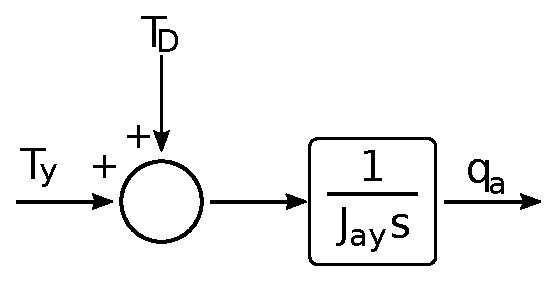
\includegraphics[width=0.44\textwidth]{Contenido/Cuerpo/Capitulo3/Fig21.eps}
	\captionof{figure}{Representación de la ecuación de movimiento en el eje Pitch}
	\label{fig:ModeloMat:Fig1}
\end{center}
Donde el término $\tau_D$ entra como disturbio al sistema
\begin{equation}
	\tau_D = (J_{az} - J_{ax})p_ar_a + D_{xz}(p^2_a - r^2_a) - D_yz(\dot{r}_a - p_aq_a)-D_{xy}(\dot{p}_a + q_ar_a)
\end{equation}

\subsection{Rotación sobre Yaw}
En la figura 3.12 podemos observar que B coincide con K para $v_1 = 0$. Asociado con esas rotaciones
tenemos las siguientes transformaciones, donde la transformación de K respecto a B fue antes descrita en la ecuación (3.14)
\begin{equation}
	L_{KB} =
	\begin{bmatrix}
		cos(v_1)  & sin(v_1) & 0 \\
		-sin(v_1) & cos(v_1) & 0 \\
		0         & 0        & 1
	\end{bmatrix}
\end{equation}
\begin{equation}
	L_{AK} =
	\begin{bmatrix}
		cos(v_2) & 0 & -sin(v_2) \\
		0        & 1 & 0         \\
		sin(v_2) & 0 & cos(v_2)
	\end{bmatrix}
\end{equation}
La ecuación (3.34) representa la transformación del marco de referencia del pitch[A] respecto a yaw[K].\\
El momento angular del sistema es la suma del momento angular de las rotaciones
de Pich y Yaw \cite{Paper::Yoon2001}\\
El momento angular del sistema está dada por $J\omega$ donde J es la matriz de inercia y $\omega$
es la velocidad angular, por lo tanto con las matrices (3.21) y (3.25) y las velocidades (3.20)
obtenemos
\begin{equation}
	H =
	\begin{bmatrix}
		H_x \\
		H_y \\
		H_z
	\end{bmatrix}
	=
	\begin{bmatrix}
		J_{kx}p_k + d_{xy}q_k + d_{yz}r_k \\
		d_{xy}p_k + J_{ky}q_k + d_{yz}r_k \\
		d_{xz}p_k + d_{yz}q_k + J_{kz}r_k
	\end{bmatrix}
	% \end{equation}
	% \begin{equation}
	+L^T_{AK}
	\begin{bmatrix}
		J_{ax}p_a + D_{xy}q_a + D_{yz}r_a \\
		D_{xy}p_a + J_{ay}q_a + D_{yz}r_a \\
		D_{xz}p_a + D_{yz}q_a + J_{az}r_a
	\end{bmatrix}
\end{equation}
El momento angular de la ecuación (3.35) es la suma del yaw y pitch expresado en el marco de
referencia de Yaw.\\
Podemos aplicar de manera similar que en Pitch las ecuaciones (3.23) (3.24) y (3.26) para
encontrar el torque total, después de algunos cálculos algebraicos, cuyos detalles se omiten,
y que están desarrollados en \cite{Paper::Yoon2001}
\begin{equation}
	J_k\dot{r}_k = T_z + T_{d1} + T_{d2} + T_{d3}
\end{equation}
Donde
\begin{equation}
	J_k = J_{kz} + J_{ax}sin^2(v_2) + J_{az}cos^2(v_2)- D_{xz}
	sin(2v_2)
\end{equation}
\begin{equation}
	T_{d1} = [J_kx + J_{ax}cos^2(v2) + J_{az}sin^2(v_2) +
			D_{xz}sin(2v_2)-(J_{ky} + J_{ay})]p_kq_k
\end{equation}
\begin{equation}
	T_{d2} = -[d_{xz} + (J_{az} - J_{ax})sin(v_2)cos(v_2)+
	D_{xz}cos(2v_2)] x (\dot{p}_k - q_kr_k)
\end{equation}
\begin{equation}\nonumber
	-(d_{yz} + D_{yz}cos(v_2) - D_{xy}sin(v_2))(\dot{q}_k + p_kr_k)
\end{equation}
\begin{equation}\nonumber
	-(d_{xy} + D_{xy}cos(v_2) + D_{yz}sin(v_2))(p^2_k - q^2_k)
\end{equation}

\begin{equation}
	T_{d3} = \ddot{v}_2(D_{xy}sin(v_2)-D_{yz}cos(v_2))
\end{equation}
\begin{center}
	$+ \dot{v}_2[(J_{ax}-J_{az})(p_kcos(2_v2)-r_ksin(2v_2))$
\end{center}
\begin{center}
	$+2D_{xz}(p_ksin(2v_2)+r_kcos(2v_2))$
\end{center}
\begin{center}
	$
	+(D_{yz}sin(v_2) + D_{xy}cos(v_2))(q_a+q_k) - J_{ay}p_k]
	$
\end{center}
Podemos tomar a $\tau_{d1}$, $\tau_{d2}$, $\tau_{d3}$ como disturbios que entran al sistema. De manera similar que en Pitch haremos algunas suposiciones, donde decimos que
la expresión (3.29) y (3.30) también son aplicables para la ecuación 3.36.
\begin{equation}
	D_{xy} = D_{xz} = D_{yz} = 0
\end{equation}
\begin{equation}
	J_{ax} = J_{az}
\end{equation}
Además, si los productos de la inercia del gimbal en Yaw también pueden ser despreciados, es decir si
\begin{equation}
	d_{xy} = d_{xz} = d_{yz} = 0
\end{equation}
Por lo que ahora obtenemos 
\begin{equation}
	J_k = J_{kz} + J_{az}
\end{equation}
\begin{equation}
	T_{d1} = [J_{kx} + J_{ax} - (J_ky + J_ay)]p_kq_k
\end{equation}
\begin{equation}
	T_{d2} = 0
\end{equation}
\begin{equation}
	T_{d3} = -J_{ay} \dot{v}_2p_k
\end{equation}
Podemos incluso seguir eliminando disturbios de entrada, haciendo que
\begin{equation}
	J_{kx} + J_{ax} = J_{ky}
\end{equation}
Dando como resultado
\begin{equation}
	T_d = T_{d1} + T_{d2} + T_{d3}
\end{equation}
\begin{equation}
	T_d = J_{ay}(p_kq_k - p_k\dot{v}_2)
\end{equation}
Entre el marco de referencia B y K tenemos la rotación $v_1$ sobre el eje z, podemos obtener de \cite{Book:Barfoot2020} la relación (3.51)
\begin{equation}
	\begin{bmatrix}
		p_k\\
		q_k\\
		r_k
	\end{bmatrix}
	=L_{KB}
	\begin{bmatrix}
		p\\
		q\\
		r
	\end{bmatrix}
	+
	\begin{bmatrix}
		0\\
		0\\
		\dot{v}_1
	\end{bmatrix}
\end{equation}
Desarrollando (3.48) tenemos
\begin{equation}\nonumber
	p_k=pcos(v_1) + qsin(v_1)
\end{equation}
\begin{equation}
	q_k = -psin(v_1) + qcos(v_1)
\end{equation}
\begin{equation}\nonumber
	r_k= r + \dot{v}_1
\end{equation}
De manera similar, entre el marco de referencia Yaw [K] y el Pitch [A] tenemos
\begin{equation}\nonumber
	p_a = p_kcos(v_2) - r_ksin(v_2)
\end{equation}
\begin{equation}
	q_a = q_k + \dot{v}_2
\end{equation}
\begin{equation}\nonumber
	r_a = p_ksin(v_2) + r_kcos(v_2)
\end{equation}
Hasta aquí hemos obtenido una ecuación de movimiento para Yaw en el marco de referencia K, es decir $r_k$. Sin embargo la salida es la velocidad angular $r_a$ es decir
la velocidad de rotación en el eje "y" respecto al marco de referencia A, por lo que las ecuaciones 3.53 nos ayudan a obtener la relación de $r_a$ y $r_k$.\\
EL diagrama de bloques de la ecuación de movimiento de Yaw se puede observar en la figura 3.14
\begin{center}
	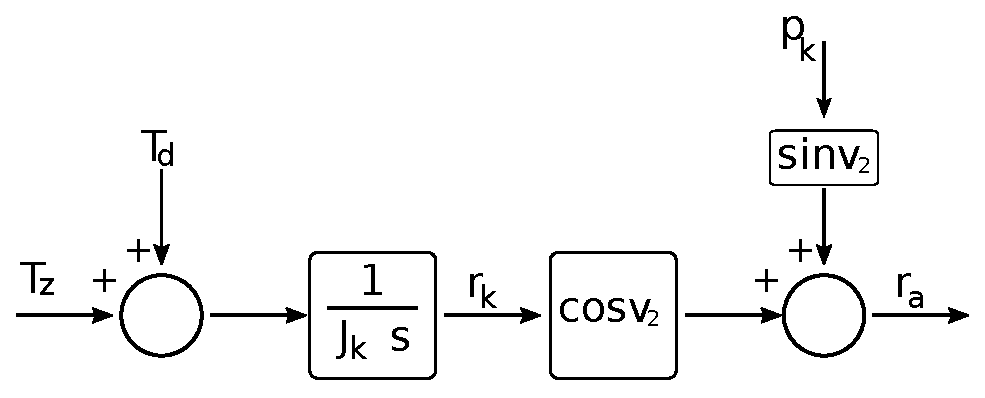
\includegraphics[width=0.7\textwidth]{Contenido/Cuerpo/Capitulo3/Fig22.eps}
	\captionof{figure}{Representación de la ecuación de movimiento en Yaw}
	\label{fig:ModeloMat:Fig1}
\end{center}


% ---------------------------------------------------------------------------------------------------------
% *********************************************************************************************************
% *********************************************************************************************************
% % ---------------------------------------------------------------------------------------------------------
% \section{Modelo matemático del motor DC}
% El mecanismo móvil del sistema esta conformado por un par de motores de corriente directa.
% La figura 3.12 muestra el diagrama electrico de un motor de corriente directa
% \begin{center}
% 	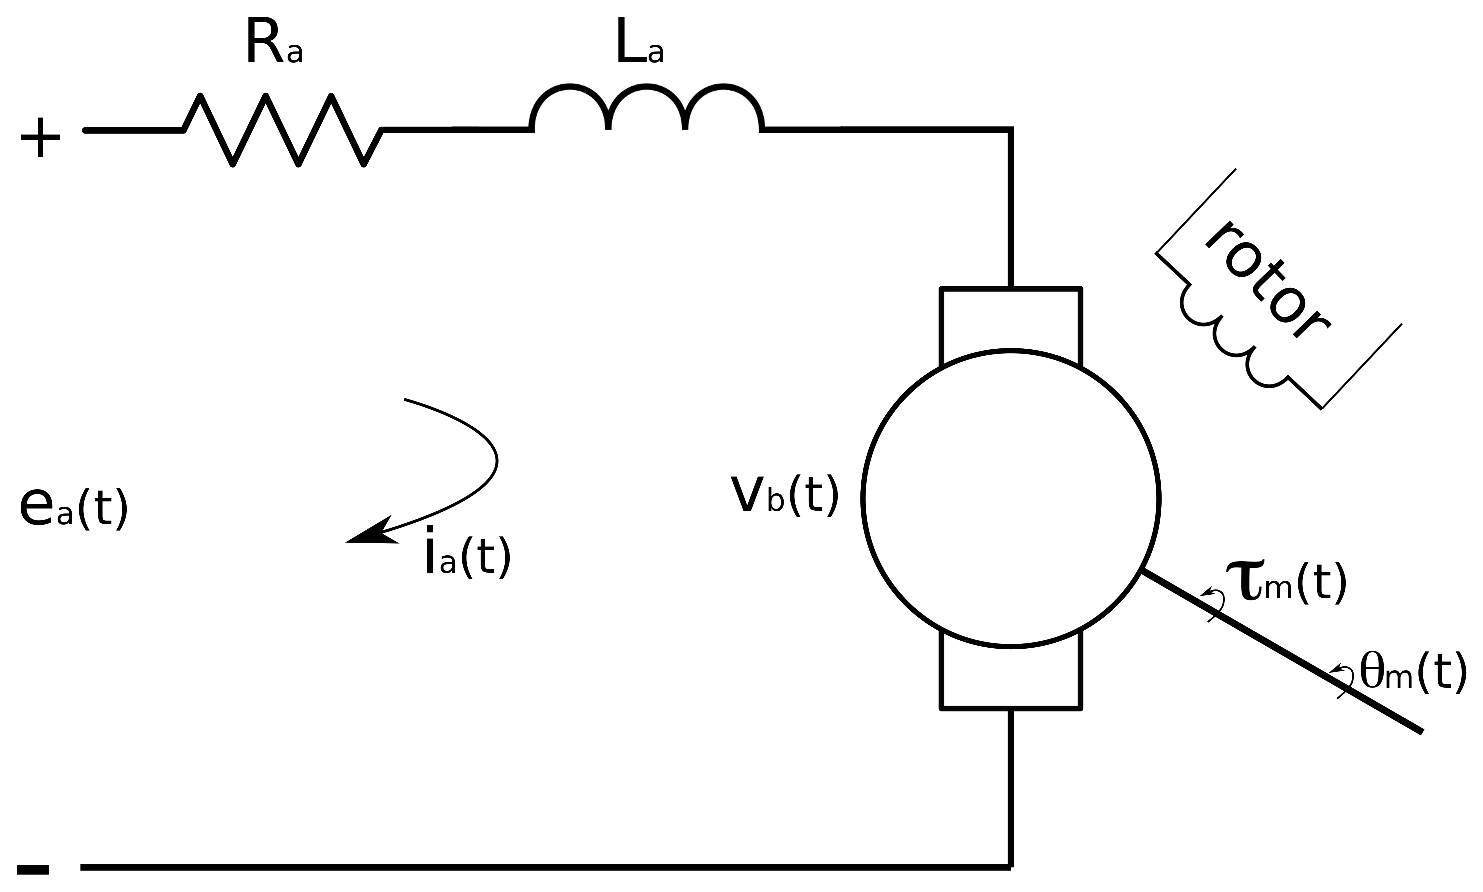
\includegraphics[width=0.5\textwidth]{Contenido/Cuerpo/Capitulo3/Fig16.eps}
% 	\captionof{figure}{Diagrama electrico de motor de corriente directa}
% 	\label{fig:ModeloMat:Fig1}
% \end{center}
% Tenemos que la fuerza contra motriz $v_b$ es igual a la expresión de la ecuación 3.54
% \begin{equation}
% 	v_b(t) =K_b \frac{d\theta_m(t)}{dt}
% \end{equation}
% donde
% \begin{itemize}
% 	\item $ \frac{d\theta_m(t)}{dt} $ = $ \omega_m(t) $
% \end{itemize}
% Aplicamos laplace a la ecuación 3.54
% \begin{equation}
% 	V_b(s) = K_bS\Theta_m(s)
% \end{equation}
% Aplicando la ley de Kirkoff a la red eléctrica de la figura 3.15 obtenemos
% \begin{equation}
% 	R_aI_a(s) + L_aSI_a(s) + V_b(s) = E_a(s)
% \end{equation}
% El torque empleado por el motor es proporcional a la corriente del inducido; por lo tanto,
% \begin{equation}
% 	\tau_m(s) = K_\tau I_a(s)
% \end{equation}
% donde $\tau_m$ es el torque del motor y $K_\tau$ es una constante de proporcionalidad, llamada constante de par del motor, que depende de las características del motor y del
% campo magnético.\\
% En un arreglo consistente de unidades, el valor de $K_t$ es igual al valor de $K_b$. Reordenando la ecuación 3.57.
% \begin{equation}
% 	I_a = \frac{1}{K_\tau} \tau_m (s)
% \end{equation}
% Para encontrar la función de transferencia del motor, primero sustituimos las ecuaciones (3.55) y (3.58) en (3.56), produciendo
% \begin{equation}
% 	\frac{(R_a + L_aS) \tau_m(s)}{K_\tau} + K_bS \Theta_m(s) = E_a(s)
% \end{equation}
% El torque del motor puede ser expresado como
% \begin{equation}
% 	\tau_m(s) = (J_mS^2 + D_mS) \Theta_m(s)
% \end{equation}
% $J_m$ es la inercia equivalente en la armadura e incluye tanto la inercia de la armadura como la inercia de carga reflejada en la armadura. $D_m$ es la amortiguación viscosa
% equivalente en la armadura e incluye tanto la amortiguación viscosa de la armadura como la amortiguación viscosa de la carga reflejada en la armadura.\\
% Sustituyendo $\tau_m$ en la ecuación 3.54 obtenemos
% \begin{equation}
% 	\frac{(R_a + L_aS) (J_mS^2 + D_mS) \Theta_m(s) }{K_\tau} + K_bS \Theta_m(s) = E_a(s)
% \end{equation}
% Si suponemos que la inductancia de la armadura, $L_a$, es pequeña en comparación con la resistencia de la armadura, $R_a$, que es habitual para un motor de corriente continua,
% la ecuación. (3.61) se convierte
% \begin{equation}
% 	\left[ \frac{R_a }{K_\tau} (J_mS^2 + D_mS) + k_b \right] S\Theta_m(s)  = E_a(s)
% \end{equation}
% Después de la simplificación, se encuentra que la función de transferencia deseada,
% \begin{equation}
% 	\frac{\theta_m (s)}{E_a(s)} = \frac{K_t / (R_aJ_m)}{s \left[ s + \frac{1}{J_m} \left( D_m + \frac{K_tK_b}{R_a} \right) \right]}
% \end{equation}
% Que en manera simple se obtiene.
% \begin{equation}
% 	\frac{\theta_m (s)}{E_a(s)} = \frac{K}{s(s+\alpha)}
% \end{equation}
% Discutamos primero las constantes mecánicas, $J_m$ y $D_m$. Considere la siguiente figura, que muestra un motor con inercia $J_a$
% y amortiguación $D_a$ en la armadura que impulsa una carga que consiste en inercia $J_L$ y amortiguación $D_L$
% \begin{center}
% 	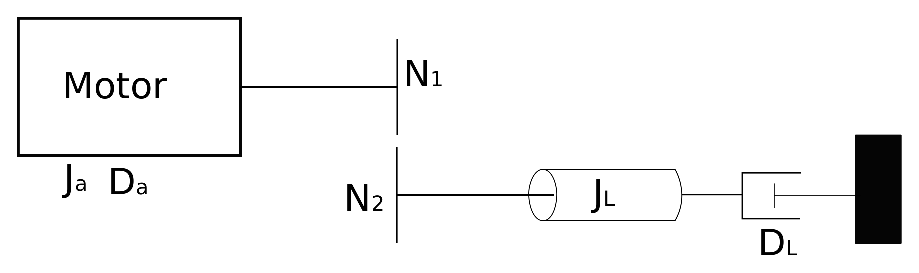
\includegraphics[width=0.5\textwidth]{Contenido/Cuerpo/Capitulo3/Fig18.eps}
% 	\captionof{figure}{Motor DC que acciona una carga mecánica rotacional}
% 	\label{fig:ModeloMat:Fig1}
% \end{center}
% Suponiendo que se conocen todos los valores de inercia y amortiguación mostrados, $J_L$ y $D_L$ pueden reflejarse de nuevo en la
% armadura como una inercia y amortiguación equivalentes para agregarse a $J_a$ y $D_a$, respectivamente. Por lo tanto, la inercia
% equivalente, $J_m$, y la amortiguación equivalente, $D_m$, en la armadura son
% \begin{subequations}
% 	\begin{equation}
% 		J_m = J_a + J_L \left( \frac{N_1}{N_2} \right)
% 	\end{equation}
% 	\begin{equation}
% 		D_m = D_a + D_L\left( \frac{N_1}{N_2} \right)
% 	\end{equation}
% \end{subequations}
% Ahora que hemos evaluado las constantes mecánicas, $J_m$ y $D_m$, tenemos que obtener las constantes electricas vistas en la
% ecuación 3.29. Sustituyendo las ecuaciones (3.55) y (3.58) en la ecuación. (3.56), con $L_a = 0$, produce
% \begin{equation}
% 	\frac{R_a}{K_t} \tau_m (s) + K_bS\theta_m(s) = E_a(s)
% \end{equation}
% Aplicando la transformada inversa de laplace obtenemos
% \begin{equation}
% 	\frac{R_a}{K_t} \tau_m (t) + K_b\omega_m(t) = e_a(s)
% \end{equation}
% Si se aplica un voltaje de CC, $e_a$, el motor girará a una velocidad angular constante, $\omega_m$, con un torque constante,$\tau_m$.
% Por lo tanto,podemos descartar la relación funcional basada en el tiempo de la ecuación (3.67), la siguiente relación existe
% cuando el motor está funcionando en estado estable con una entrada de voltaje de CC:
% \begin{equation}
% 	\frac{R_a}{K_t} \tau_m + K_b\omega_m = e_a
% \end{equation}
% La ecuación 3.69 representa una linea recta de $\tau_m$ vs $\omega_m$
% \begin{equation}
% 	\tau_m = -\frac{K_bK_t}{R_a} \omega_m + \frac{K_t}{R_a}e_a
% \end{equation}
% Este gráfico se llama curva de par-velocidad. La intersección del eje de torque ocurre cuando la velocidad angular llega a cero.
% Ese valor de par se llama Torque "stall", $\tau_{stall}$.
% \begin{center}
% 	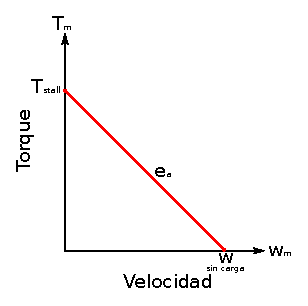
\includegraphics[width=0.45\textwidth]{Contenido/Cuerpo/Capitulo3/Fig19.eps}
% 	\captionof{figure}{Curva de par-velocidad}
% 	\label{fig:ModeloMat:Fig1}
% \end{center}
% Por tanto tenemos que
% \begin{equation}
% 	T_{stall} = \frac{K_t}{R_a}e_a
% \end{equation}
% La velocidad angular que ocurre cuando el torque es cero se llama velocidad sin carga, $\omega_{sin carga}$ . Así,
% \begin{equation}
% 	\omega_{sin carga} = \frac{e_a}{K_b}
% \end{equation}
% Las constantes eléctricas de la función de transferencia del motor ahora se pueden encontrar en las ecuaciones (3.70) y (3.71) como
% \begin{equation}
% 	\frac{K_t}{R_a} = \frac{T_{stall}}{e_a}
% \end{equation}
% y
% \begin{equation}
% 	K_b = \frac{e_a}{\omega_{sincarga}}
% \end{equation}